\documentclass{article}
\usepackage{amsfonts}
\usepackage{amsthm}
\usepackage{amssymb}
\usepackage{amsmath}
\usepackage{graphicx}
\usepackage{subcaption}
\usepackage{xcolor}
\usepackage{mathtools}
\usepackage{ wasysym }
\usepackage{enumerate}
\usepackage{verbatim}


\numberwithin{equation}{section}
\newcommand{\new}[2]{
    \vspace{2mm}
    \noindent
    \textbf{
    \underline{#1}}
    \textit{{#2}}
    \
}

\def\<{{\langle}}
\def\>{{\rangle}}

\DeclarePairedDelimiter\bra{\langle}{\rvert}
\DeclarePairedDelimiter\ket{\lvert}{\rangle}
\DeclarePairedDelimiterX\braket[2]{\langle}{\rangle}{#1\,\delimsize\vert\,\mathopen{}#2}


\newcommand{\textOr}{
    {
        \hspace{5mm}
        \textrm{or}
        \hspace{5mm}
    }
}

\newcommand{\textAnd}{
    {
        \hspace{5mm}
        \textrm{and}
        \hspace{5mm}
    }
}


\newcommand{\textWhere}{
    {
        \hspace{5mm}
        \textrm{where}
        \hspace{5mm}
    }
}



\newcommand{\Ixp}[1]{
    {
        e^{i{#1}}
    }
}



\newcommand{\halfFigure}[1]{
\begin{center}
\includegraphics[width = .5\linewidth]{{#1}}
\end{center}
}

\newcommand{\fullFigure}[1]{
\begin{center}
\includegraphics[width = .9\linewidth]{{#1}}
\end{center}
}

\def\twobytwoMat(#1, #2, #3, #4){
    {
        \begin{bmatrix}
            {#1} & {#2}\\
            {#3} & {#4}
        \end{bmatrix}
    }
}

\def\twobyoneMat(#1, #2){
    {
        \begin{bmatrix}
            {#1}\\
            {#2}
        \end{bmatrix}
    }
}

\def\twobytwoDet(#1, #2, #3, #4){
    {
        \begin{vmatrix}
            {#1} & {#2}\\
            {#3} & {#4}
        \end{vmatrix}
    }
}


\newcommand{\RR}{\mathbb{R}}
\newcommand{\CC}{\mathbb{C}}
\newcommand{\ZZ}{\mathbb{Z}}
\newcommand{\Zpos}{\mathbb{Z}_{pos}}
\newcommand{\NN}{\mathbb{N}}

\newcommand{\deriv}[2]{
\frac {d {#1} } {d {#2}}
}

\newcommand{\pderiv}[2]{
\frac {\partial {#1} } {\partial {#2}}
}

\newtheorem{theorem}{Theorem}
\newtheorem{proposition}{Proposition}
\newtheorem{lemma}{Lemma}
\newtheorem{corollary}{Corollary}
\newtheorem{remark}{Remark}
\newtheorem{definition}{Definition}
\newtheorem{example}{Example}
\newtheorem{conjecture}{Conjecture}
\newtheorem{question}{Question}

\newcommand{\ch}{\text{ch}}

\begin{document}
\begin{center}
    \Large
    \textbf{411T Midterm}

    \large
    Daniel Son
\end{center}

\section{Falling Stick}
\begin{figure}[htp]
    \centering
    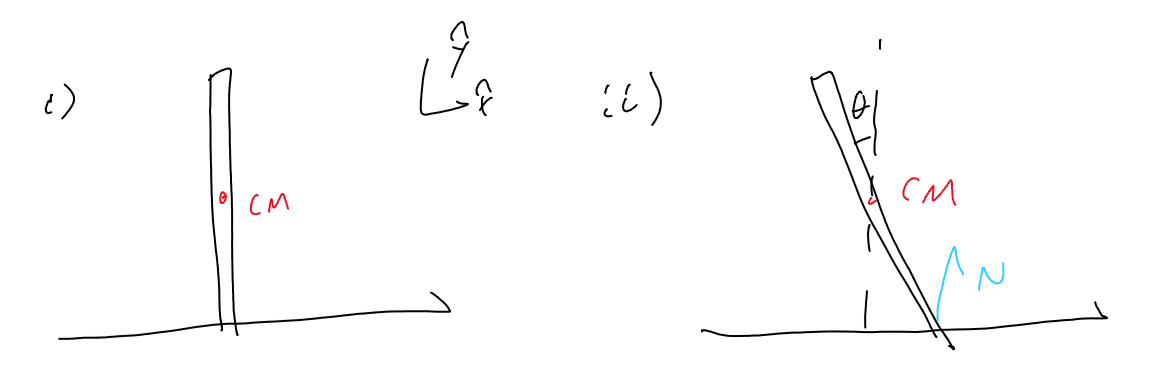
\includegraphics[width=0.8\textwidth]{Q1_figure.png} % Replace 'figure.jpg' with your image file
    \caption{Setup for Q1, the length of the rod is $2l$, and 
    $\theta$ is the angular displacement measured CCW from the vertical.}
    \label{fig:q1setup}
\end{figure}

\begin{proof}[Part a]
    In order to compute the potential $U$, we must consider the conservative forces 
    acting on the rod. The gravitational force exerts a fixed force of 
    of $-mg \hat y$. 

    Set the potential at the surface to be zero. The potential 
    of the system is a linear equation with respect to the height $y$. 
    \begin{align}
        U(x, y) \ = \ mg y
    \end{align}\footnote{$y \neq \hat y$. The former is the height, the 
    latter is a unit vector pointing upwards. }
    \begin{figure}[h]
        \centering
        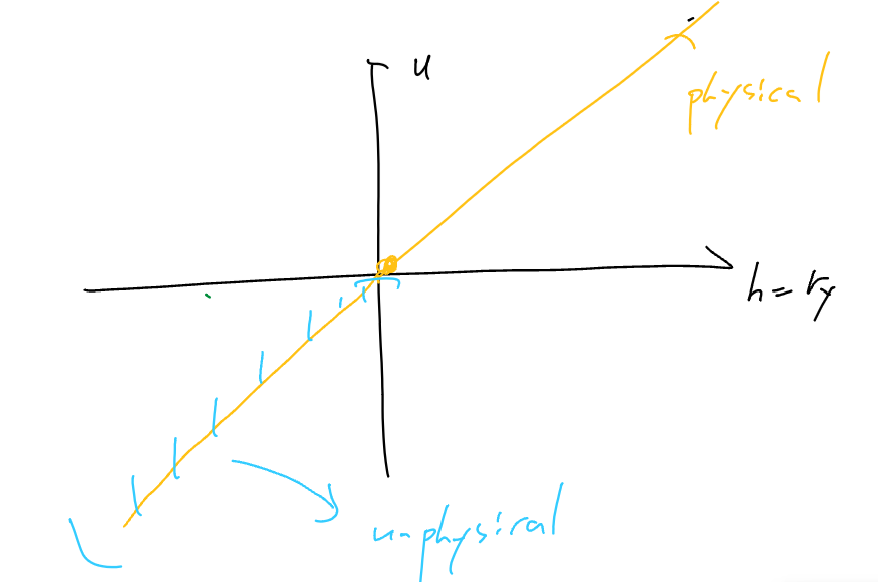
\includegraphics[width=0.8\textwidth]{Q1_Potential.png} % Replace 'figure.jpg' with your image file
        \caption{A sketch of the potential. $r_y = y$}
        \label{fig:q1potential}
    \end{figure}
    We note that the cases where $y < 0$ is unphysical, since the object 
    is bound to exist over the surface. 
\end{proof}

\begin{remark}
    We note that the forces acting on the rod is entirely parallel 
    to the $y$-axis. Hence, the motion of the rod is characterized 
    by one parameter, either height or the angular displacement from the vertical. 
    The relationship between the two parameters are 
    \begin{align}
        y \ = \ l \cos(\theta)
    \end{align}
\end{remark}

\begin{proof}[Part b]
    Compute the Lagrangian in terms of angular displacement, $\theta$. 
    \begin{align}
        U \ = \ mgy \ = \ mgl \cos(\theta) \\ 
        T \ = \ \frac 1 2 m \dot y^2 + \frac 1 2 I \omega^2 \ = \  
        \frac 1 2 m l^2 \sin(\theta)^2 \dot \theta^2 + \frac 1 6 m l^2 \dot\theta^2 
        \ = \ \frac 1 2 m l^2 \dot \theta^2 \left(
            \sin(\theta)^2 + \frac 1 3
        \right)\\\boxed{
        \mathcal L \ = \ T - U \ = \ 
        \frac 1 2 m l^2 \dot \theta^2 \left(
            \sin(\theta)^2 + \frac 1 3
        \right) - 
         mgl \cos(\theta)}
    \end{align}

    Apply the Lagrange equation wrt the angular displacement.  
    \begin{align}
        \pderiv {\mathcal L} {\theta} \ = \ \deriv{}{t} \pderiv{\mathcal L}{\dot \theta} 
    \end{align}
    Faithfully applying the derivatives, we obtain the following. 
    \begin{align}
        m l^2 \dot \theta^2 \sin(\theta) \cos(\theta) + mgl \sin(\theta) \ = \ \deriv{}{t} m l^2 \dot \theta^2 (\sin(\theta)^2 + 1/3) \\ 
        \dot \theta ^2 \sin(\theta) \cos(\theta) + \frac g l \sin(\theta) \ = \ \ddot \theta (\sin(\theta)^2 + 1/3) + \dot\theta^2 (2 \sin(\theta) \cos(\theta)) \\ 
        \boxed{\ddot \theta \ = \ \frac{3g \sin(\theta) - 3l\dot\theta^2 \sin(\theta)\cos(\theta)}{3l\sin(\theta)^2 + l}}
    \end{align}
\end{proof}

\begin{proof}[Part c]
    Lets use Newtonian mechanics to solve for $\ddot \theta$. 
    We obtain an equation for force and torque. 
    \begin{figure}[htp]
        \centering
        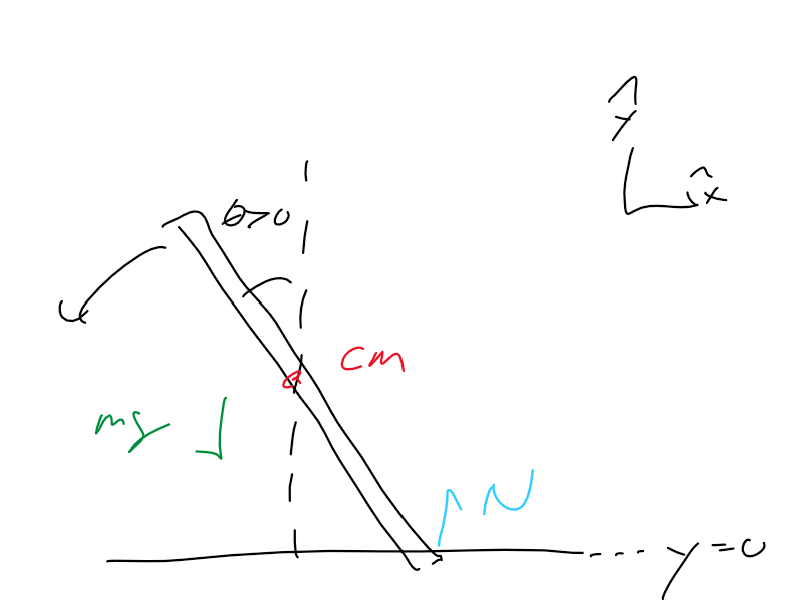
\includegraphics[width=0.8\textwidth]{Q1_FBD.png} % Replace 'figure.jpg' with your image file
        \caption{Diagram with force labels}
        \label{fig:example}
    \end{figure}
    
    \begin{align}
        \sum F = -mg + N \ = \ m \ddot y \\ 
        \tau \ = \ I \alpha \ = \ \frac{ml^2} 3 \ddot \theta \ = \ N l \sin(\theta)
    \end{align}
    Solving for $N$ and canceling out redundant terms, we obtain 
    \begin{align}\label{eqn:q1a}
        l\ddot \theta \ = \ 3 g \sin(\theta) - 3 l \ddot \theta \sin(\theta)^2 - 3 l \dot\theta^2 \sin(\theta)\cos(\theta) \\ 
        \boxed{\ddot \theta \ = \ \frac{
            3 g \sin(\theta) - 3 l \dot \theta^2 \sin(\theta) \cos(\theta)
        } {3l \sin(\theta)^2 + l}}
    \end{align}
    which is great, since the result agrees with Part c. 
\end{proof} 
\footnote{Thanks for answering my questions, pf Jensen, pf Strauch. It helped a lot. }

\begin{proof}[Part d]
    Use conservation of energy to compute the value of $\dot \theta$. 
    \begin{align}
        E \ = \ \frac 1 2 m l^2 \dot \theta^2 \left(
            \sin(\theta)^2 + \frac 1 3
        \right) + mgl \cos(\theta) \ = \ mgl
    \end{align}
    Plug in $\theta = \pi / 2$ to get angular velocity. 
    \begin{align}
        \dot \theta_1 = \sqrt{\frac {3g}{2l}}
    \end{align}
    Angular acceleration follows from \eqref{eqn:q1a}. 
    \begin{align}
        \ddot \theta_1 \ = \ \frac {3g}{4l}
    \end{align}
    Compute linear velocity and linear acceleration by taking 
    consecutive derivatives of $y$. 
    \begin{align}\boxed{
        \dot y_1 \ = \ -l \dot \theta_1 \sin(\pi/2) \ = \ -\sqrt{\frac 3 2 gl} }\\\boxed{ 
        \ddot y_1 \ = \ -l \ddot \theta_1 \sin(\pi/2) - l \dot\theta^2_1 \cos(\pi/2) \ = \ -\frac 3 4 g}
    \end{align}
    The negative signs indicate that the velocity and acceleration points 
    towards the negative $y$-direction. 
\end{proof}


\section{Rotating Spring}
\begin{figure}[htp]
    \centering
    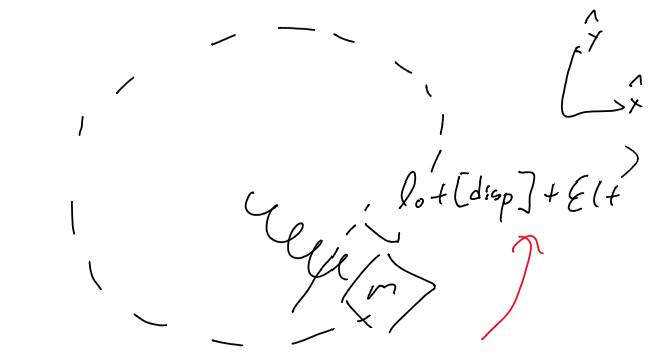
\includegraphics[width=0.8\textwidth]{Q2_figure.png} % Replace 'figure.jpg' with your image file
    \caption{Setup for Q2}
    \label{fig:q2setup}
\end{figure}

\begin{proof}[Part a]
    At equilibrium, the centrepetal force matches the force 
    exerted by the string. 
    \begin{align}
        \frac {m v^2} r \ = \ kx
    \end{align}
    Rewrite the velocity and displacement in terms of $r, \phi$. 
    \begin{align}
        x \ = \ r - l_0 \\ 
        v \ = \ \dot\phi (l_0 + x)
    \end{align}
    Solve for $x$. Also, $\dot \phi = \omega$ constantly. 
    \begin{align}
        \frac{m \dot \phi^2 (l_0 + x)^2} {l_0 + x} \ = \ kx \\ 
        m \dot \phi^2 (l_0 + x) \ = \ kx \\ 
        x \ = \ \frac {m \omega^2 l_0} {k - m \omega^2}\\
        \boxed{
            r_0 \ = \ l_0 + x \ = \ \frac{k l_0}{k - m \omega^2} 
        }
    \end{align}
\end{proof}

\begin{proof}[Part b]
    To compute the Lagrangian, we compute the kinetic and potential energy. 
    Recall that 
    \begin{align}
        v \ = \ \sqrt{\dot r^2 + r^2 \dot \phi^2}.
    \end{align}
    Write out $T, U$. 
    \begin{align}
        T & = \ \frac 1 2 mv^2 \ = \ \frac 1 2 m (\dot r^2 + r^2 \dot \phi^2) \\ 
        U & = \ \frac 1 2 k (r - l_0)^2
    \end{align}
    Thus 
    \begin{align}
        \mathcal L(t, r, \dot r, \phi, \dot \phi)  \ = \ T - U \ = \  
        \frac 1 2 \left(
            m (\dot r^2 + r^2 \dot \phi^2) - k(r - l_0)^2
        \right).
    \end{align}
    Faithfully apply the Lagrange equation for both the radial and 
    angular displacement. 
    \begin{align}
       \pderiv{\mathcal L}{r} \ = \ \deriv{}{t} \pderiv{\mathcal L} {\dot r} 
       \textOr 
       m r \dot \phi^2 - k(r - l_0)  \ = \ \deriv{}{t} m \dot r \nonumber \\ \textOr 
       \boxed{\ddot r \ = \ \left(\dot\phi^2 - \frac k m\right) r + \frac k m l_0}\\
       \pderiv{\mathcal L}{\phi} \ = \ \deriv{}{t} \pderiv{\mathcal L}{\dot \phi} 
       \textOr 0 \ = \ \deriv{}{t} (mr^2\dot\phi) \nonumber\\ 
       \boxed{
        2 r\dot r \dot \phi + r^2 \ddot \phi = 0
       }
    \end{align}
\end{proof}
    
\begin{proof}[Part c]
    Set $r(t) = r_0 + \epsilon(t)$. Also suppose $\dot \phi \approx \omega$ constantly. 
    The Lagrange equation with respect to radial displacemnt simplifies as follows. 
    \begin{align}
        \ddot \epsilon \ = \ \left(
            \omega^2 - \frac k m 
        \right) (r_0 + \epsilon) + \frac k m l_0  \ = \ 
        \left(
            \frac{m \omega^2 - k}{m} 
        \right)\left(
            \frac {k l_0} {k - m \omega^2} + \epsilon
        \right) + \frac k m l_0 \ \nonumber \\ = \ 
        - \frac k m l_0 + \frac k m l_0 + \left(
            \omega^2 - \frac k m
        \right)\epsilon \ = \ \left(
            \omega^2 - \frac k m
        \right)\epsilon \\ 
        \boxed{
            \ddot \epsilon \ = \ \left(
                \omega^2 - \frac k m 
            \right)\epsilon
        }
    \end{align} 
    Assuming $\omega^2 - k/m < 0$, $\epsilon$ is a solution for 
    a simple harmonic oscillator. A particular solution for 
    $\epsilon(0) = A, \dot \epsilon (0 ) = 0$ is 
    \begin{align}
            \epsilon(t) \ = \ A \cos\left(\sqrt{\frac k m - \omega^2}\right)
    \end{align}
    Thus
    \begin{align}
        \boxed{
            \Omega \ = \ \sqrt{\frac k m - \omega^2}
        }.
    \end{align}
\end{proof}


\begin{proof}[Part d]
        Without the assumption  $\omega^2 - k/m < 0$, $\epsilon$ displays 
    exponential decay. Under the initial condition $\epsilon(0) = A$, 
    a particular solution is 
    \begin{align}
        \epsilon(t) \ = \ \frac {A e^{-qt} + B e^{+qt}} 2 
    \end{align}
    where
    \begin{align}
        q \ = \ \sqrt{
            \omega^2 - \frac k m
        }
    \end{align}
    Physically, it is not plausible that $\epsilon$ displays exponential growth. 
    Thus, we set $B = 0$
    We write the solution in one clean formula. 
    \begin{align}
        \boxed{
            \epsilon(t) \ = \ A \exp\left(
                -t\sqrt{\omega^2 - \frac k m}
            \right)
        }
    \end{align}
    The formula tells us that the displacement of the spring reaches 
    the equilibrium position in an asymptotic manner as $t \rightarrow \infty$. 
\end{proof}

\begin{proof}[Part e]
    We investigate the change of $\phi$ over time. From the 
    Lagrange equation w.r.t. angular displacement, solve for $\ddot \phi$. 
    \begin{align}
        \ddot \phi \ = \ - 2 \frac {\dot r} r \dot \phi 
    \end{align}
    Set $\dot \phi_0 \ = \ \omega$. Then, apply the method of successive 
    approximations. 
    \begin{align}
        \ddot \phi_1 \ = \ - 2 \frac {\dot r} r \dot \phi_0 \ = \ - 2 \omega \frac {\dot r} r \ = \ \frac {2 \omega q} {r_0} A e^{-tq}
    \end{align}
    Suppose $\phi(\infty) = \omega$. Then, 
    \begin{align}
        \dot \phi_1 \ = \ \omega + C e^{-qt}
    \end{align}\footnote{The exact expression of constant $C$ is not of our interest. }
    satisfies the differential equation and the limiting condition. 
    \textcolor{blue}{
        Regardless of the initial amplitude of the oscillation, the angular velocity will display exponential 
        decay either from above or below and reach a constant terminal velocity of $\omega$. 
    }
\end{proof}

\section{Modeling Matter}
\begin{proof}[Part a]
    \begin{figure}[h]
        \centering
        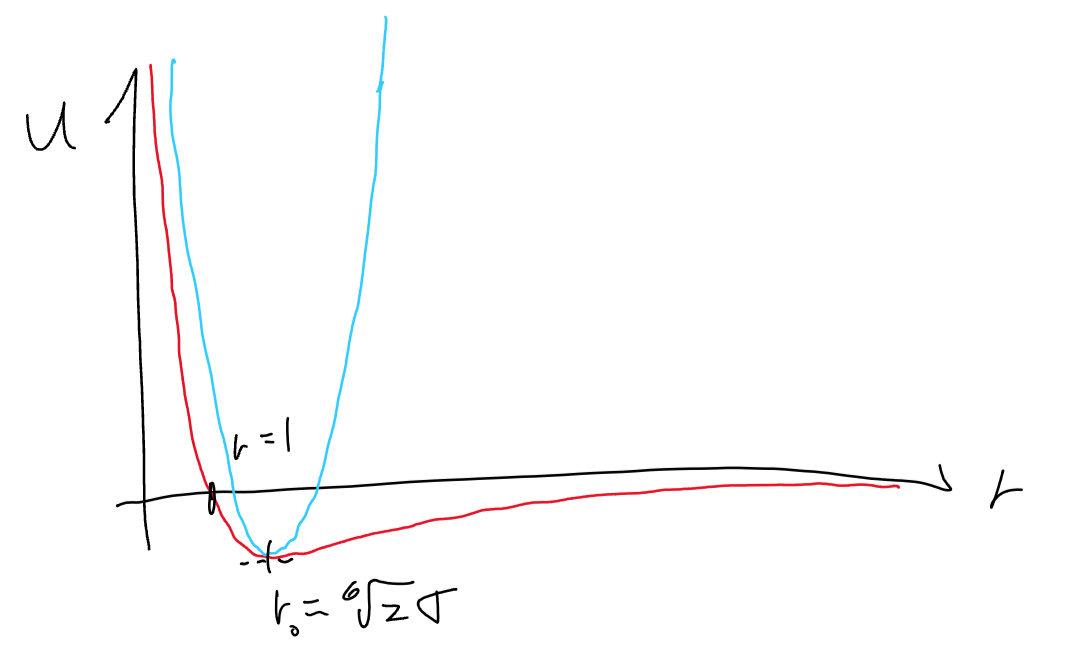
\includegraphics[width=0.8\textwidth]{Q3_Potential.png} % Replace 'figure.jpg' with your image file
        \caption{Plot of $U(r)$ with "stiffer spring" potential. The potential 
        at the valley is $-\epsilon$. \textcolor{red}{Also, the potential reaches 
        zero at $r = \sigma$, not 1}. }
        \label{fig:q3plot}
    \end{figure}
    \begin{figure}[h]
        \centering
        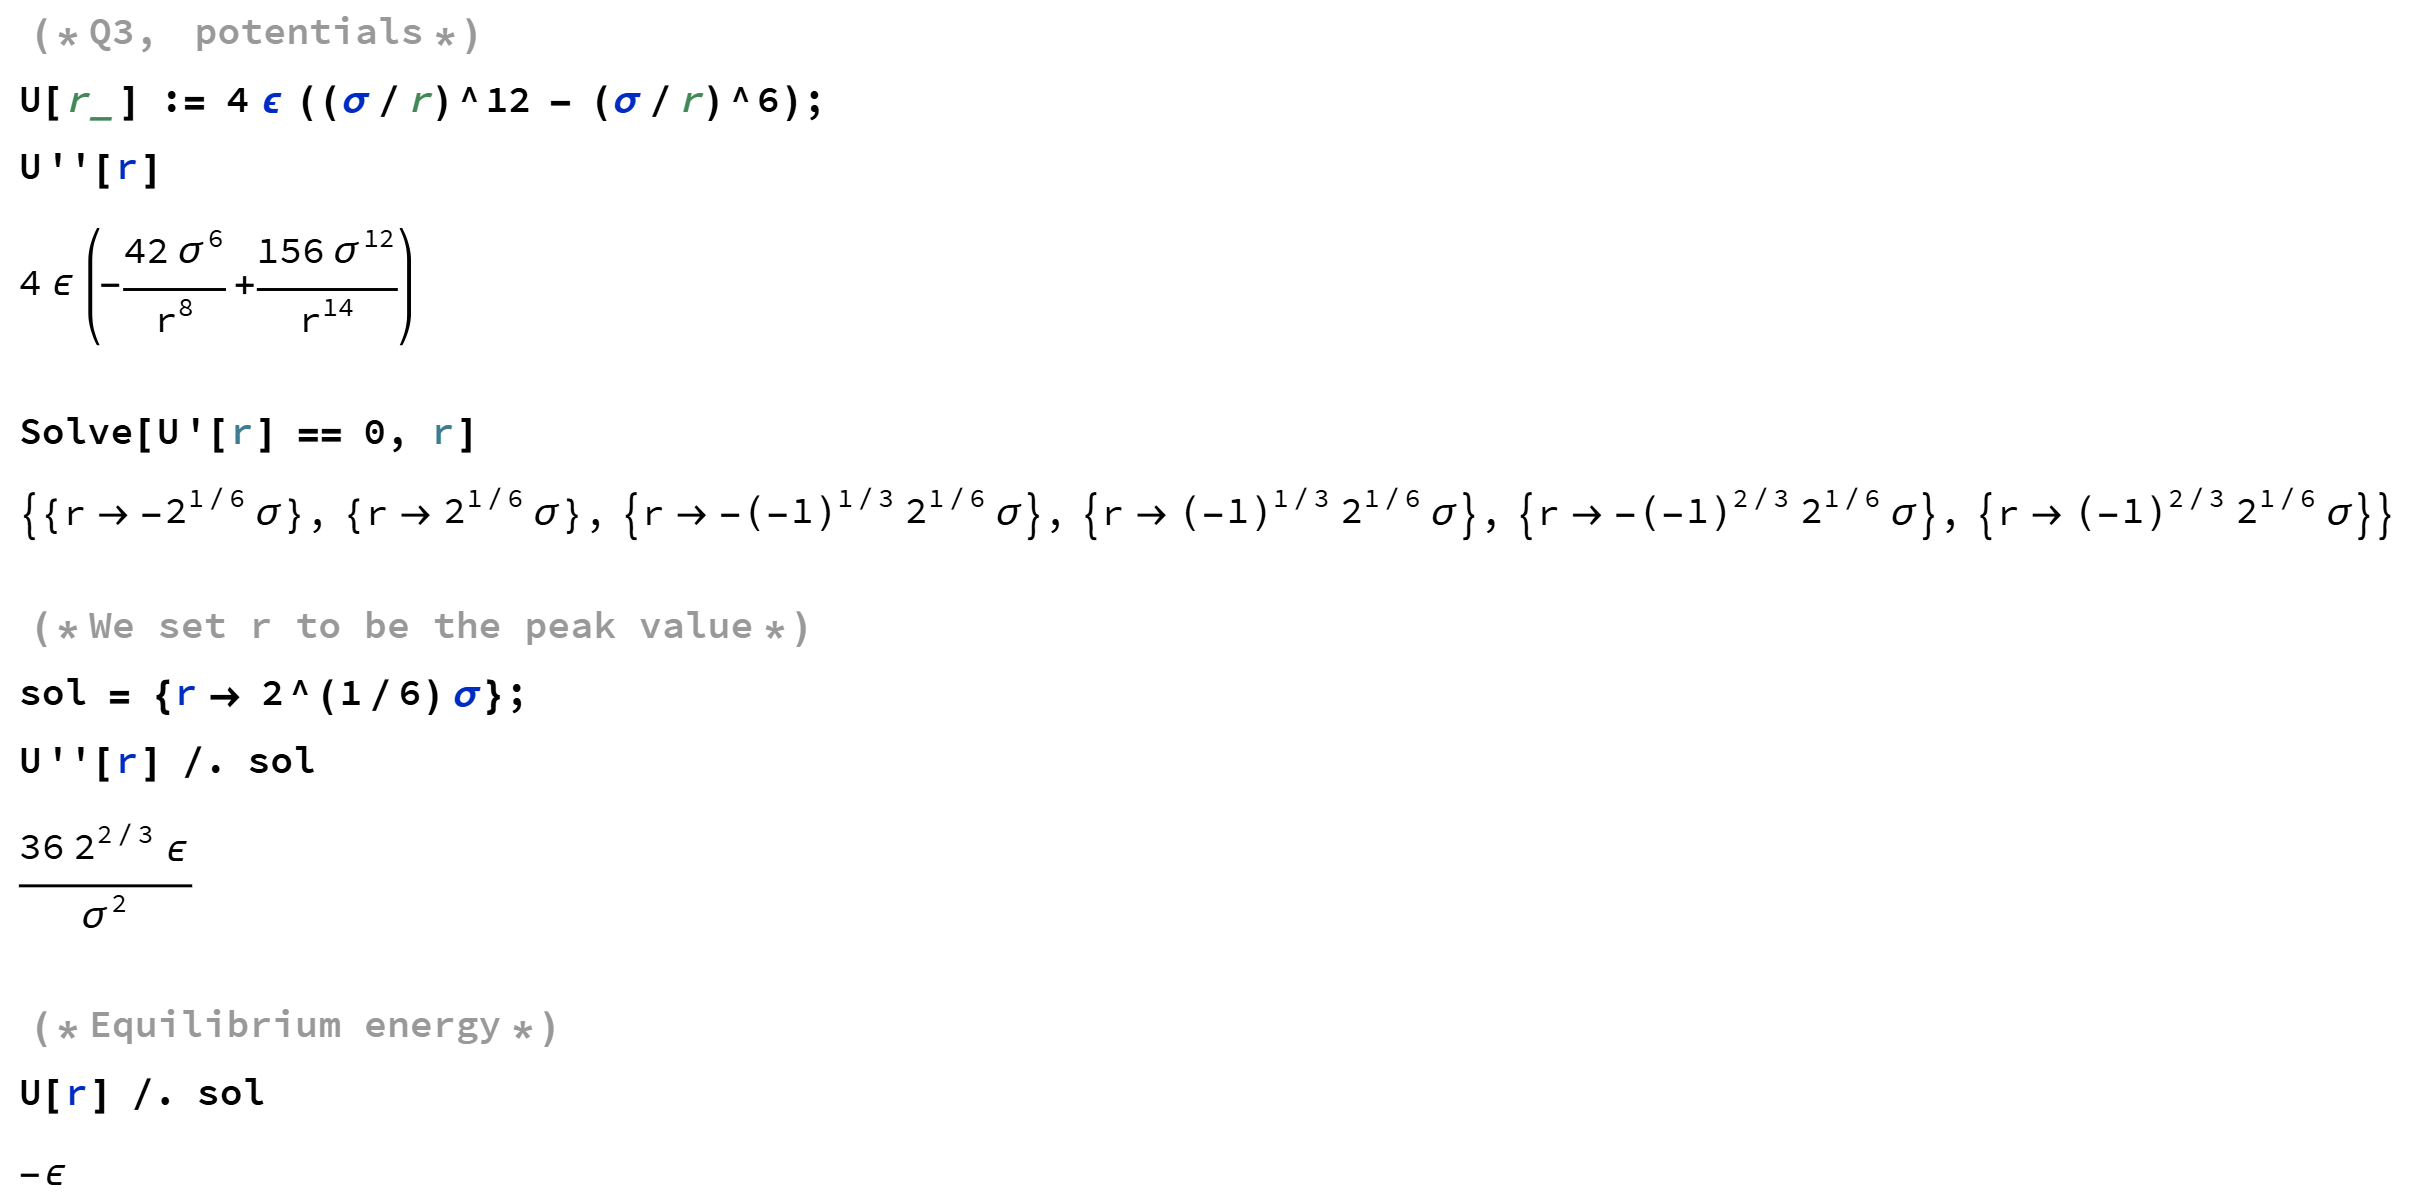
\includegraphics[width=0.8\textwidth]{Q3_code.png} % Replace 'figure.jpg' with your image file
        \caption{Supplemental Mathematica code}
        \label{fig:q3code}
    \end{figure}
    
    The stationary point is attained when $\deriv{U}{r} = 0$. With the 
    help of mathematica, we notice that the equilibrium position is 
    \begin{align}
        r_0 \ = \ 2^{1/6} \sigma
    \end{align}
    and 
    \begin{align}
        U(r_0) \ = \ -\epsilon
    \end{align}.
    Upon inspection, we recognize tht the potential reaches zero at $r = \sigma$. 
    \begin{align}
        U(\sigma) \ = \ 0
    \end{align}
\end{proof}

\begin{proof}[Part b]
    The effective spring constant is the value of the second derivative 
    of the potential at the valley. Mathematica computation shows the following. 
    \begin{align}
        U''(r_0) \ = \ \frac {36 \cdot 2^{2/3} \epsilon} {\sigma^2}
    \end{align}
    \textcolor{blue} {Thus, the spring constant increases for higher $\epsilon$ 
    and lesser $\sigma$}. 
\end{proof}

\begin{proof}[Part c]
    We notice that for $E \geq 0$, the motion of the particle is unbounded. 
    For $E < 0$, the horizontal energy limit must intersect with the 
    potential, since $\lim_{r \rightarrow \infty}U(r) = 0$, and for 
    this case, the particle is bounded. We expect small oscilaltions 
    around the valley, i.e. $E \approx -\epsilon$. \footnote{E must be 
    slightly greater than $\epsilon$, since negative kinetic energy is not allowed. } 
\end{proof}

\begin{proof}[Part d]
\end{proof}
\begin{figure}[htp]
    \centering
    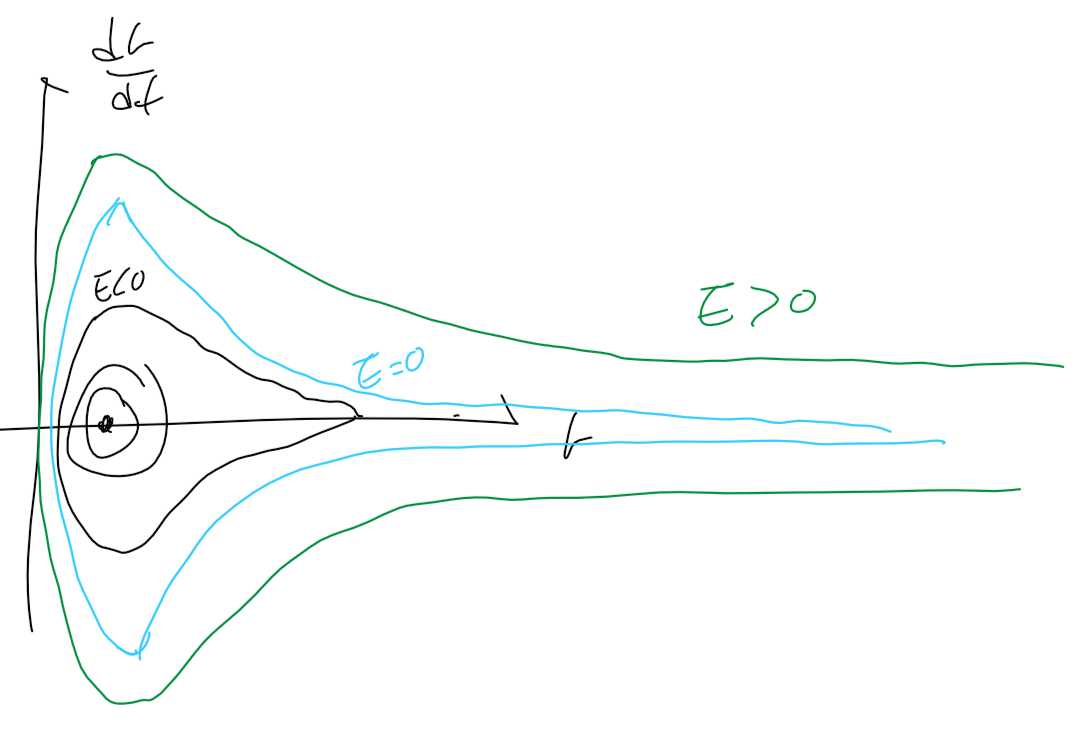
\includegraphics[width=0.8\textwidth]{Q3_PhaseDiagram.png} % Replace 'figure.jpg' with your image file
    \caption{Phase space diagram. Particle is bounded for 
    trajectories corresponding to $E<0$. For particles with $E \geq 0$, 
    the trajectories display unbounded behavior. The center dot is a stationary trajectory with $E = -\epsilon$. }
    \label{fig:q3phaseSpace}
\end{figure}

\section{Bending Light}
\begin{proof}[Part a]
    Fermat's principle states that the ray of light follows 
    the trajectory which takes the minimal amount of time to 
    travel between two points. We set up an integral to describe 
    time elapsed between two points. 
    \begin{align}
        t \ = \ \int_1^2 \frac {n(y) ds}c \ = \ 
        \frac 1 c \int_{0}^{x_t} \left(1 + \frac {y(x)} l\right)
        \sqrt{1 + y'(x)^2} dx
    \end{align}
    We wish to apply calculus of variations. We set up our function 
    $f$ as follows. 
    \begin{align}
        f(x, y, y') \ = \ \left(1 + \frac y l\right) \sqrt{1 + y'(x)^2}
    \end{align}
    The function $f$ has no explicit $x$ dependency. Hence, we apply 
    Beltrami's identity. Suppose $C$ is a constant. 
    \begin{align}
        f - y' \pderiv f {y'} \ = \ C \\ 
        f - y' \left(1 + \frac y l \right) \frac {2 y'} {2 \sqrt{1 + y'^2}} \ = \ C \\ 
        \frac {1 + y/l}{\sqrt{1 + y'^2}} = C
    \end{align}
    We solve for $y'$ and apply seperation of variables to obtain an equation 
    of $x$ with respect to $y$. 
    \begin{align}
        y'(x) \ = \ \sqrt{
            \left(
                \frac 1 C + \frac y {Cl}
            \right)^2 - 1
        } \\ 
        x \ = \ \int_{y_0}^{y_t} \frac {dy} {\sqrt{
            \left(
                \frac 1 C + \frac y {Cl}
            \right)^2 - 1}}
    \end{align}
    Apply $u$-substitution where $u$ is the quantity within the parentheses. 
    \begin{align}
        x \ = \ \int_{y_0/Cl + 1/C}^{y_t/Cl + 1/C} \frac {Cl du} {\sqrt{u^2 - 1}} 
        \\ 
       x \ = \ Cl \tanh^{-1}\left(
            \frac {u} {\sqrt{u^2 - 1}}
        \right) \bigg|_{y_0/Cl + 1/C}^{y_t/Cl + 1/C}
    \end{align}
    Solving for $y_t$, we deduce that the solution must be in the following form. 
    \begin{align}
        \boxed{
        y_t\ = \ y(x)  \ = \ C l \cosh\left(
            \frac x {Cl} + B
        \right) - l}
    \end{align}
    Imposing $y(0) = y_0$ and $y'(0) = y'_0$, we compute $B, C$
    \begin{align}
        C \ = \ \frac{y_0/l + 1 }{\sqrt{1 + {y'}_0^2}} \\ 
        B \ = \ -\cosh^{-1}\left(\sqrt{1 + {y'}_0^2}\right)
    \end{align}
\end{proof}

\begin{proof}[Part b]
    Upon inspection, the reflection point occurs when the argument 
    of the $\cosh$ function vanishes. This occurs in the following 
    value of $x$. 
    \begin{align}\label{eqn:x0exact}
        \boxed{
        x_0 \ = \ -lBC \ = \  
            \frac{y_0 + l }{\sqrt{1 + {y'}_0^2}}\cosh^{-1}\left(\sqrt{1 + {y'}_0^2}\right)
        }
    \end{align}
\end{proof}

\begin{proof}[Part c]
    Taylor expand the following two functions for $x \ll 1$. 
    \begin{align}
        \cosh(x) \ \approx \ 1 + \frac {x^2} 2 \\ 
        \sqrt{1 + x^2} \ \approx \ 1 + \frac {x^2} 2
    \end{align}
    So, for $x \ll 1$, 
    \begin{align}
        \cosh^{-1}\left(\sqrt{1 + x^2}\right) \ \approx \ x 
    \end{align}
    which leads us to approximate \eqref{eqn:x0exact} as 
    \begin{align}
        \boxed{
        x_0 \ = \ (y_0 + l) (y'_0)}
    \end{align}

    
    
\end{proof}


\end{document}